% Atividade XIII -- Estratégias de crescimento, viabilidade e coerência
% Compilação: pdflatex -> bibtex -> pdflatex -> pdflatex
\documentclass[12pt, a4paper, article, oneside, brazil]{abntex2}
% Preâmbulo comum às Atividades XII e XIII (classe abnTeX2, modo artigo).
% Normas: ABNT NBR 14724:2024, NBR 10520:2023, NBR 6023:2018, NBR 6024:2012,
% NBR 6027:2012, NBR 6028:2021.
\usepackage{lmodern}
\usepackage[T1]{fontenc}
\usepackage[utf8]{inputenc}
\usepackage{indentfirst}
\usepackage{microtype}
\usepackage{graphicx}
\usepackage{booktabs}
\usepackage{longtable}
\usepackage{array}
\usepackage{tabularx}
\usepackage{xcolor}
\usepackage{tikz}
\usetikzlibrary{positioning, arrows.meta}
\usepackage{amsmath}
\usepackage{pgfplots}
\pgfplotsset{compat=1.16}
\usepackage[alf]{abntex2cite}
\usepackage{hyperref}

\setlrmarginsandblock{3cm}{2cm}{*}
\setulmarginsandblock{3cm}{2cm}{*}
\checkandfixthelayout
\OnehalfSpacing
\setlength{\parindent}{1.25cm}
\setlength{\parskip}{0pt}
\renewcommand{\arraystretch}{1.25}
\captiondelim{ -- }
\newcommand{\fontsizetable}{\footnotesize}
\newcommand{\fonteautores}{\par\vspace{2pt}{\footnotesize Fonte: elaborado pelos autores (2026).}\par}
\newcommand{\fontetexto}[1]{\par\vspace{2pt}{\footnotesize Fonte: #1.}\par}
\newcommand{\projeto}{PetCuida}
\newcolumntype{L}[1]{>{\raggedright\arraybackslash}p{#1}}
\newcolumntype{Y}{>{\raggedright\arraybackslash}X}

\hypersetup{
  colorlinks=true, linkcolor=black, citecolor=black, urlcolor=black, breaklinks=true,
  pdfauthor={Gabriel da Silva Cassino; Giovanna Naves Ribeiro; Júlia Rodrigues Vasconcellos Melo; Kathleen Rodrigues Leite Barbosa},
  pdfsubject={Tópicos III -- Empreendedorismo e Inovação}
}
\urlstyle{same}

% Uso: \capadocumento{TÍTULO EM CAIXA ALTA}{subtítulo}
\newcommand{\capadocumento}[2]{%
\begin{capa}
  \begin{center}
    
\includegraphics[width=0.25\textwidth]{images/brasao.png}\par
    \vspace{0.4cm}
    {\large\textbf{PONTIFÍCIA UNIVERSIDADE CATÓLICA DE MINAS GERAIS}}\par
    Campus Coração Eucarístico\par
    Curso de Engenharia de Computação\par
    Disciplina: Tópicos III -- Empreendedorismo e Inovação\par
    \vspace{1.6cm}
    Gabriel da Silva Cassino\par
    Giovanna Naves Ribeiro\par
    Júlia Rodrigues Vasconcellos Melo\par
    Kathleen Rodrigues Leite Barbosa\par
    \vfill
    {\Large\textbf{#1}}\par
    \vspace{0.3cm}
    {\large #2}\par
    \vfill
    Belo Horizonte\par
    2026
  \end{center}
\end{capa}}
\newcommand{\folharosto}[3]{%
\begin{folhaderosto}
  \begin{center}
    Gabriel da Silva Cassino\par
    Giovanna Naves Ribeiro\par
    Júlia Rodrigues Vasconcellos Melo\par
    Kathleen Rodrigues Leite Barbosa\par
    \vspace{3cm}
    {\Large\textbf{#1}}\par
    \vspace{0.3cm}
    {\large #2}\par
    \vspace{2cm}
  \end{center}
  \hspace{.45\textwidth}
  \begin{minipage}{.5\textwidth}
    \begin{SingleSpace}
      \small
      Trabalho acadêmico em grupo apresentado à disciplina Tópicos III -- Empreendedorismo e Inovação, do Curso de Engenharia de Computação da Pontifícia Universidade Católica de Minas Gerais, como requisito parcial de avaliação referente à #3.\par
      \vspace{0.4cm}
      Professor-orientador: Prof. João Carlos Oliveira Caetano\par
      Professor-tutor: Prof. Paulo Mattos
    \end{SingleSpace}
  \end{minipage}
  \vfill
  \begin{center}
    Belo Horizonte\par
    2026
  \end{center}
\end{folhaderosto}}

\hypersetup{pdftitle={Atividade XIII: estratégias de crescimento, viabilidade e coerência},
  pdfkeywords={crescimento; escalabilidade; startup; plataforma; viabilidade}}

\begin{document}
\selectlanguage{brazil}
\frenchspacing
\capadocumento{ESTRATÉGIAS DE CRESCIMENTO, VIABILIDADE E COERÊNCIA}{Atividade XIII -- Startup \projeto}
\folharosto{ESTRATÉGIAS DE CRESCIMENTO, VIABILIDADE E COERÊNCIA}{Atividade XIII -- Startup \projeto}{Atividade XIII}
\begin{resumo}[RESUMO]
\begin{SingleSpace}
\noindent Este documento apresenta o plano de crescimento e escalabilidade da startup PetCuida, plataforma digital de prevenção e acesso a cuidados para animais de companhia. O diagnóstico situa o negócio na fase de validação inicial, ainda sem receita nem usuários pagantes, e identifica como principais desafios a disposição a pagar não medida, a dependência de convênios para o resultado positivo, o custo do fundo de liquidação de créditos solidários, que supera a contribuição unitária, o custo de aquisição não mensurado e o arranque simultâneo dos dois lados da plataforma. Propõem-se duas estratégias de crescimento: a densidade local por meio de parcerias com clínicas e organizações, expandindo-se por praças somente após gatilhos mensuráveis, e o aprofundamento de receita com novos serviços condicionados a evidências. As ações de escalabilidade abrangem automação, uso de tecnologia, modelo replicável por praça e receita recorrente. Uma simulação baseada na economia unitária da Atividade IX mostra que a escala, por si só, é insuficiente: a contribuição de R\$~0,55 por usuário ativo por mês só se torna robusta com alavancas combinadas. O plano termina com quadro de ação, metas, indicadores e uma análise explícita de viabilidade e coerência.

\vspace{\onelineskip}
\noindent\textbf{Palavras-chave}: startup; estratégia de crescimento; escalabilidade; plataforma de dois lados; economia unitária.
\end{SingleSpace}
\end{resumo}

\clearpage
\pagenumbering{roman}
\tableofcontents*
\clearpage
\pagenumbering{arabic}
\setcounter{page}{1}
\section{Introdução}
\label{sec:introducao}

A Atividade XIII solicita um plano de crescimento e escalabilidade para o projeto de startup do grupo, considerando o momento atual do negócio e as oportunidades de mercado \cite{pucminas2026xiii}. A orientação organiza o trabalho em quatro etapas: diagnóstico do estágio atual, duas estratégias de crescimento, estratégias de escalabilidade e plano de ação resumido com recursos e indicadores. Este documento segue essa ordem (Seções~\ref{sec:diagnostico} a \ref{sec:plano}) e acrescenta uma seção de viabilidade e coerência (Seção~\ref{sec:coerencia}), em atenção ao título da atividade.

O plano apoia-se nas atividades anteriores: o protótipo e os testes com usuários \cite{grupo2026a6}, os canais prioritários \cite{grupo2026a8}, o levantamento de custos e a precificação \cite{grupo2026a9}, o tipo societário \cite{grupo2026a10} e a estrutura organizacional \cite{grupo2026a11}. Em particular, os valores numéricos de custos, preços e receitas provêm da Atividade IX, que os classifica como estimativas do grupo e hipóteses a validar. Esses valores são reproduzidos aqui com essa mesma ressalva, e a simulação do Apêndice~A permite que o grupo substitua as premissas por dados reais assim que o piloto os produzir.

Dois princípios orientam o texto. O primeiro é a distinção entre crescer e escalar: crescer é aumentar clientes ou receita, mesmo à custa de custos proporcionalmente maiores; escalar é aumentar clientes ou receita sem crescimento proporcional dos custos, conforme a orientação. O segundo é a coerência: uma estratégia só é recomendada se for compatível com o estágio do negócio, com a economia unitária, com os canais já definidos e com a capacidade de uma equipe de quatro integrantes.

\section{Diagnóstico do estágio atual}
\label{sec:diagnostico}

\subsection{Fase do negócio}

A \projeto{} encontra-se na fase de \textbf{validação}, em estágio inicial e anterior à tração. O \textit{Startups Report Brasil 2024}, do Observatório Sebrae Startups, mostra que 33,45\% das startups mapeadas estão em validação e que apenas 3,72\% se encontram na etapa de escala \cite{sebrae2025estagios}; a \projeto{} integra, portanto, o grupo mais numeroso do ecossistema, e o aprendizado de validação é seu principal ativo neste momento. A Tabela~\ref{tab:evidencias} reúne as evidências que sustentam esse diagnóstico.

\begin{table}[htb]
\centering
\caption{Evidências do estágio de validação}
\label{tab:evidencias}
\fontsizetable
\begin{tabularx}{\textwidth}{L{3.3cm} Y}
\toprule
\textbf{Dimensão} & \textbf{Situação atual}\\
\midrule
Produto & Protótipo funcional (versão \textit{Alpha 3i}) com cadastro e histórico do animal, calendário de vacinas, prontuário com código QR, triagem orientativa, rede solidária e agendamento; dados locais e demonstrativos, sem pagamentos reais, notificações ou geolocalização \cite{cassino2026repo}. Há ainda aplicação web temporária e arquivos de instalação para teste.\\
Evidência com usuários & Cinco sessões de demonstração guiada com perfis distintos, com recepção favorável e sugestões de melhoria, sobretudo quanto à clareza do sistema de créditos \cite{grupo2026a6}. Não houve execução autônoma de tarefas, e a disposição a pagar das classes C, D e E ainda não foi medida \cite{grupo2026a9}.\\
Receita e clientes & Sem receita, sem usuários pagantes e sem clínicas contratadas. Os valores de receita são projeções do grupo.\\
Formalização & Proposta de constituição como sociedade empresária limitada com quatro sócios \cite{grupo2026a10}; empresa ainda não constituída.\\
Equipe & Quatro integrantes com frentes e substitutos definidos \cite{grupo2026a11}.\\
\bottomrule
\end{tabularx}
\fonteautores
\end{table}

\subsection{Principais desafios para o crescimento}

\begin{table}[htb]
\centering
\caption{Desafios para o crescimento, evidências e implicações}
\label{tab:desafios}
\fontsizetable
\begin{tabularx}{\textwidth}{L{0.7cm} L{3.4cm} Y Y}
\toprule
\textbf{N.º} & \textbf{Desafio} & \textbf{Evidência} & \textbf{Implicação para o plano}\\
\midrule
1 & Disposição a pagar não medida & O teste de aceitação do preço está planejado, mas não realizado \cite{grupo2026a9}. & Validar preço do PetCuida+ e do Plano Parceiro antes de ampliar o investimento em aquisição.\\
2 & Dependência de convênios & Sem os R\$~1.500,00 mensais de convênio e patrocínio, o resultado do cenário enxuto é de R\$~$-$653,68 no mês 12 \cite{grupo2026a9}. & Contratar ao menos um convênio ou patrocínio é condição para a sustentabilidade inicial.\\
3 & Fundo de liquidação de créditos & O fundo custa R\$~6,60 por atendimento, valor superior à margem de R\$~5,24 do atendimento antes do fundo; a margem após o fundo é de R\$~$-$1,36 \cite{grupo2026a9}. & Reduzir o fundo (patrocínio de campanhas, limites de uso) é pré-requisito da escala.\\
4 & Custo de aquisição não medido & O CAC não foi observado; os R\$~150,00 mensais de divulgação não comprovam CAC baixo \cite{grupo2026a9}. & Medir o CAC no piloto e adotar um teto de gasto por usuário (Subseção~\ref{sub:cac}).\\
5 & Arranque de dois lados & Tutores só valorizam a plataforma se houver clínicas, e clínicas só pagam se houver tutores \cite{rochet2003,eisenmann2006}. & Concentrar a oferta numa praça pequena e subsidiar o lado mais sensível a preço.\\
6 & Segurança e dados pessoais & O protótipo ainda não está pronto para dados reais; a LGPD exige base legal e consentimento \cite{brasil2018lgpd}. & Endurecer a segurança e formalizar privacidade antes do piloto com usuários reais.\\
7 & Capacidade da equipe & Quatro integrantes com outras obrigações; conhecimento técnico concentrado \cite{grupo2026a11}. & Limitar o número de frentes simultâneas e manter revisão em dupla.\\
\bottomrule
\end{tabularx}
\fonteautores
\end{table}

\section{Estratégias de crescimento}
\label{sec:crescimento}

\subsection{Critérios de escolha}

A orientação sugere considerar expansão de mercado, lançamento de novos produtos ou serviços, parcerias estratégicas e estratégias de marketing e aquisição. A matriz de produto e mercado de \citeonline{ansoff1957} distingue quatro direções de crescimento: penetração de mercado, desenvolvimento de mercado, desenvolvimento de produto e diversificação. Dado que a \projeto{} ainda não penetrou nenhum mercado e opera com recursos escassos, a diversificação foi descartada. As demais opções foram avaliadas segundo quatro critérios de viabilidade, apresentados na Tabela~\ref{tab:opcoes}.

\begin{table}[htb]
\centering
\caption{Avaliação das opções de crescimento}
\label{tab:opcoes}
\fontsizetable
\begin{tabularx}{\textwidth}{L{2.7cm} L{2.0cm} L{2.2cm} L{2.2cm} Y}
\toprule
\textbf{Opção} & \textbf{Custo inicial} & \textbf{Aderência à fase de validação} & \textbf{Exigência da equipe} & \textbf{Efeito na economia unitária}\\
\midrule
Parcerias com clínicas e ONGs & Baixo & Alta & Média & Positivo: cada clínica paga R\$~79,90 por mês e traz atendimentos.\\
Expansão geográfica (nova praça) & Médio & Média & Alta & Neutro até haver densidade; risco de diluir esforço.\\
Marketing e aquisição de tutores & Baixo a médio & Média & Média & Depende do CAC, ainda não medido.\\
Novos produtos e serviços & Médio & Baixa a média & Alta & Positivo só se aumentar assinatura ou reduzir o fundo.\\
\bottomrule
\end{tabularx}
\fonteautores
\end{table}

Com base nessa avaliação, definem-se duas estratégias que se reforçam mutuamente: a Estratégia 1, de densidade local por meio de parcerias (principal), e a Estratégia 2, de aprofundamento de receita e novos serviços (complementar).

\subsection{Estratégia 1 (principal): densidade local por meio de parcerias}

\textbf{Descrição.} Em plataformas de dois lados, o valor para cada lado depende da presença do outro, e o arranque exige conquistar ambos \cite{rochet2003}. \citeonline{eisenmann2006} recomendam decidir qual lado subsidiar e por quanto tempo. Na \projeto{}, o lado subsidiado é o tutor, cujo núcleo é gratuito, e o lado pagante inclui as clínicas (Plano Parceiro) e os patrocinadores. A estratégia consiste em concentrar o esforço em Belo Horizonte e em sua região metropolitana, construindo densidade de clínicas e tutores em poucas áreas antes de abrir novas praças. A capital integra o grupo das dez cidades com mais startups do país, o que favorece o acesso a parceiros e a talentos \cite{diario2025bh}.

\textbf{Componentes.}
\begin{alineas}
  \item \textit{Parcerias}: três clínicas no piloto, com três meses gratuitos do Plano Parceiro, e organizações não governamentais e lideranças comunitárias como porta de entrada dos tutores, com a faculdade de medicina veterinária como possível apoio à curadoria da triagem;
  \item \textit{Aquisição}: os três canais prioritários de comunicação e de distribuição da Atividade VIII \cite{grupo2026a8}, a saber, redes sociais, parcerias com clínicas e indicação, e código QR no balcão das clínicas e lojas oficiais de aplicativos, com programa de indicação remunerado em créditos;
  \item \textit{Expansão por praça}: abrir uma nova área apenas quando os gatilhos da Tabela~\ref{tab:gatilhos} forem atingidos.
\end{alineas}

\begin{table}[htb]
\centering
\caption{Gatilhos para abrir uma nova praça}
\label{tab:gatilhos}
\fontsizetable
\begin{tabularx}{\textwidth}{L{5.2cm} Y}
\toprule
\textbf{Gatilho} & \textbf{Referência}\\
\midrule
Pelo menos 10 clínicas ativas e 1.500 usuários ativos mensais na praça atual & Premissas do mês 12 da Atividade IX\\
Custo de aquisição observado igual ou inferior ao teto & Subseção~\ref{sub:cac}\\
Pelo menos 5\% dos usuários assinando o PetCuida+ & Premissa da Atividade IX\\
Fundo de liquidação por atendimento igual ou inferior a R\$~6,60, com trajetória de queda & Tabela~\ref{tab:alavancas}\\
Convênio ou patrocínio contratado & Dependência do resultado positivo\\
\bottomrule
\end{tabularx}
\fonteautores
\end{table}

\subsection{Estratégia 2 (complementar): aprofundamento de receita e novos serviços}

\textbf{Descrição.} Em termos da matriz de Ansoff, trata-se de desenvolvimento de produto para o mesmo mercado. A estratégia atua sobre as três fontes de receita já definidas e sobre o principal ponto fraco do modelo, o fundo de liquidação. Seus componentes são: (i) realizar o teste de aceitação do preço e elevar a conversão ao PetCuida+ de 5\% para 8\% dos usuários; (ii) vender campanhas patrocinadas que financiem parte do fundo, objetivo de reduzi-lo de R\$~6,60 para R\$~3,30 por atendimento; (iii) ampliar o Plano Parceiro, com agenda e destaque no mapa; e (iv) acrescentar novos serviços somente quando houver evidência de demanda.

\textbf{Novos serviços candidatos.} Os testes de usabilidade registraram sugestões espontâneas de adoção, controle de alimentação e comparação de preços em lojas parceiras \cite{grupo2026a6}. Esses itens entram em lista de espera e só são desenvolvidos se, após a validação do núcleo, houver demanda recorrente de usuários e se o custo de desenvolvimento for coberto por receita ou patrocínio. Essa regra evita a dispersão de uma equipe pequena, risco apontado na Atividade XI.

\subsection{Relação entre as estratégias}

A Estratégia 1 gera os usuários e as clínicas sem os quais a Estratégia 2 não tem base de conversão; a Estratégia 2 gera a margem que torna sustentável a expansão da Estratégia 1. A sequência é, portanto, simultânea e interdependente: o piloto (Estratégia 1) fornece os dados para o teste de preço e para a venda de patrocínio (Estratégia 2).

\section{Estratégias de escalabilidade}
\label{sec:escalabilidade}

\subsection{O que limita a escala hoje}

A escalabilidade de uma plataforma depende de a receita adicional de cada novo usuário superar o custo adicional de atendê-lo. A Tabela~\ref{tab:unitaria} decompõe, a partir das premissas da Atividade IX, a economia de um usuário ativo mensal no cenário-base, sem convênios.

\begin{table}[htb]
\centering
\caption{Economia por usuário ativo mensal no cenário-base (R\$/mês)}
\label{tab:unitaria}
\fontsizetable
\begin{tabularx}{\textwidth}{Y L{3.0cm}}
\toprule
\textbf{Linha} & \textbf{Valor por usuário}\\
\midrule
Receita: comissão de intermediação (10\% dos atendimentos, 10\% dos usuários) & 0,77\\
Receita: assinatura PetCuida+ (5\% dos usuários) & 0,65\\
Receita: Plano Parceiro (1 clínica por 150 usuários) & 0,53\\
\textbf{Receita total} & \textbf{1,95}\\
(--) Taxas de pagamento e da loja de aplicativos & (0,32)\\
(--) Impostos (6\%) & (0,12)\\
(--) Infraestrutura e suporte & (0,30)\\
(--) Fundo de liquidação de créditos & (0,66)\\
\textbf{Contribuição por usuário ativo} & \textbf{0,55}\\
\bottomrule
\end{tabularx}
\fontetexto{cálculo dos autores a partir da Atividade IX (Apêndice A)}
\end{table}

O resultado é revelador: cada usuário adicional contribui com apenas R\$~0,55 por mês, e o fundo de liquidação de créditos (R\$~0,66 por usuário) é maior do que a contribuição líquida. Em consequência, para cobrir os custos fixos do cenário com equipe remunerada, seriam necessários cerca de 10.155 usuários ativos mensais, mesmo contando com o convênio (Atividade IX). Crescer apenas em número de usuários, sem alterar a composição da receita e do fundo, é caminho longo e frágil. As ações a seguir buscam elevar a contribuição por usuário e reduzir o custo fixo por usuário, que é a definição prática de escalar.

\subsection{Automação de processos}

\begin{table}[htb]
\centering
\caption{Processos candidatos à automação}
\label{tab:automacao}
\fontsizetable
\begin{tabularx}{\textwidth}{L{3.2cm} Y Y}
\toprule
\textbf{Processo} & \textbf{Automação proposta} & \textbf{Efeito esperado}\\
\midrule
Cadastro de clínicas e profissionais & Autocadastro de organizações e importação em lote de profissionais, funcionalidade já presente na aplicação web (até 500 linhas por arquivo) \cite{cassino2026repo}. & Onboarding de nova clínica sem trabalho manual da equipe.\\
Lembretes de vacinas e consultas & Notificações automáticas pelo calendário do animal; o custo das notificações do Firebase é nulo, segundo a Atividade IX. & Engajamento e retenção sem custo variável relevante.\\
Triagem orientativa & Fluxo por perguntas com regras fixas e encaminhamento, sem diagnóstico, com revisão veterinária da base de regras. & Menos atendimentos humanos de primeira linha.\\
Pagamentos e repasses & Conciliação automática dos pagamentos por Pix e cartão e relatório mensal de repasses às clínicas. & Menos horas de operação financeira por clínica.\\
Suporte & Ajuda e perguntas frequentes no aplicativo; respostas rápidas no WhatsApp Business para dúvidas recorrentes. & Menor custo de suporte por usuário.\\
Materiais de divulgação & Geração automática do cartaz com código QR de cada clínica a partir do cadastro. & Distribuição replicável a baixo custo.\\
\bottomrule
\end{tabularx}
\fonteautores
\end{table}

\subsection{Uso de tecnologia para ganho de eficiência}

A aplicação web da Atividade IX opera com persistência em banco SQLite, validada de ponta a ponta, e possui adaptadores para serviços remotos que ainda são esboços parciais, sem testes contra instâncias reais \cite{cassino2026repo}. A migração para um serviço gerenciado com autenticação e autorização no servidor, regras de segurança e testes de integração é, portanto, pré-requisito técnico da escala, e precede qualquer expansão de usuários. Em seguida, recomenda-se monitorar o uso e o custo de infraestrutura por usuário ativo, para verificar a premissa de R\$~0,10 por usuário por mês, e manter a suíte de testes de regressão como condição para cada liberação, de modo que o crescimento de usuários não aumente proporcionalmente o esforço de correção.

\subsection{Modelos replicáveis}

A \projeto{} é uma plataforma digital e, portanto, replicável por natureza, mas a replicação em outra cidade exige parceiros locais. Propõe-se transformar a experiência do piloto em um \textbf{pacote de praça}: lista de verificação de abertura, modelo de contrato do Plano Parceiro, \textit{kit} de divulgação com código QR, roteiro de captação de ONGs e painel de indicadores. Com o pacote, a abertura de uma nova praça passa a depender de execução padronizada e não de reinvenção. Duas formas mais avançadas de replicação foram consideradas e adiadas: o licenciamento da plataforma a prefeituras, universidades ou redes de ONGs, que só faz sentido após prova de funcionamento em ao menos uma praça, e a franquia, que exigiria marca, padronização operacional e suporte incompatíveis com o estágio atual.

\subsection{Receitas recorrentes}

As fontes de receita recorrente são o PetCuida+ (R\$~12,90 por mês ou R\$~119,00 por ano, equivalente a 23\% de desconto sobre doze mensalidades), o Plano Parceiro (R\$~79,90 por mês) e os convênios de patrocínio. No mês 12 da Atividade IX, assinaturas e plano de parceiros somam R\$~1.766,50, isto é, 40,0\% da receita estimada; com convênios renovados, a parcela recorrente sobe a 73,9\%. A comissão de intermediação (R\$~1.155,00) é receita transacional, mais sensível a sazonalidade. Priorizar o plano anual e contratos anuais com clínicas e patrocinadores aumenta a previsibilidade do caixa.

\subsection{Teto de custo de aquisição}
\label{sub:cac}

Como o custo de aquisição ainda não foi medido, o plano adota uma regra de contenção: o gasto para adquirir um usuário ativo não deve exceder a contribuição que ele gera em seis meses. No cenário-base, 6 $\times$ R\$~0,55 resulta em um teto de aproximadamente R\$~3,29 por usuário; com as alavancas combinadas (contribuição de R\$~1,42), o teto sobe para cerca de R\$~8,53. Para levar a base de 300 para 1.500 usuários entre os meses 3 e 12 (1.200 novos usuários, sem considerar perda), o gasto máximo no cenário-base seria de cerca de R\$~3.946, ou R\$~438 por mês em nove meses, valor superior aos R\$~150 mensais hoje previstos para divulgação. A diferença de cerca de R\$~288 por mês reduziria o resultado mensal do cenário enxuto de R\$~756,32 para algo próximo de R\$~468, ainda positivo desde que o convênio se confirme. O CAC efetivamente observado substituirá esta estimativa assim que houver dados.

\subsection{Simulação das alavancas}

A Tabela~\ref{tab:alavancas} mostra o efeito de cada alavanca, isolada ou combinada, sobre a contribuição por usuário e sobre os pontos de equilíbrio. A Figura~\ref{fig:equilibrio} compara o número de usuários necessário para o equilíbrio do cenário com equipe remunerada.

\begin{table}[htb]
\centering
\caption{Efeito das alavancas sobre a economia unitária e o ponto de equilíbrio}
\label{tab:alavancas}
\fontsizetable
\begin{tabularx}{\textwidth}{Y L{2.3cm} L{2.6cm} L{2.6cm} L{2.6cm}}
\toprule
\textbf{Alavanca (isolada, salvo indicação)} & \textbf{Contribuição por usuário (R\$/mês)} & \textbf{Equilíbrio A, sem convênio (usuários)} & \textbf{Equilíbrio B, com convênio (usuários)} & \textbf{Resultado A em 1.500 usuários (R\$/mês)}\\
\midrule
Cenário-base (Atividade IX) & 0,55 & 2.693 & 10.155 & 756,32\\
Patrocínio cobre 50\% do fundo & 0,88 & 1.681 & 6.339 & 1.251,32\\
Assinantes: 8\% dos usuários & 0,85 & 1.729 & 6.519 & 1.214,91\\
Parceiros pagantes: 1 por 100 usuários & 0,79 & 1.880 & 7.089 & 1.111,95\\
PetCuida+ a R\$~14,90 & 0,63 & 2.354 & 8.876 & 874,82\\
Três primeiras alavancas combinadas & 1,42 & 1.039 & 3.918 & 2.065,55\\
\bottomrule
\end{tabularx}
\fontetexto{simulação dos autores a partir do modelo da Atividade IX (Apêndice A); com convênio de R\$~1.500,00 por mês nas colunas 4 e 5}
\end{table}


\begin{figure}[htb]
\centering
\caption{Usuários ativos necessários para o equilíbrio do cenário B, com convênio}
\label{fig:equilibrio}
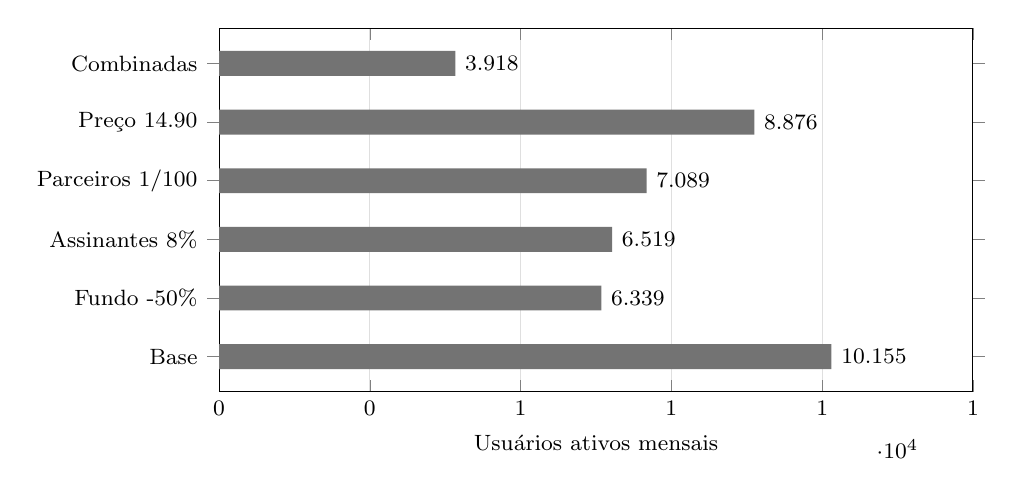
\begin{tikzpicture}
\begin{axis}[
  xbar, width=0.92\textwidth, height=6.2cm, bar width=9pt,
  xmin=0, xmax=12500, xlabel={Usuários ativos mensais},
  symbolic y coords={Combinadas,Preço 14.90,Parceiros 1/100,Assinantes 8\%,Fundo -50\%,Base},
  ytick=data, y dir=reverse,
  nodes near coords={\pgfmathprintnumber[fixed,precision=0,set thousands separator={.}]{\pgfplotspointmeta}},
  nodes near coords align={horizontal},
  every node near coord/.append style={font=\footnotesize},
  tick label style={font=\footnotesize}, label style={font=\footnotesize},
  xtick distance=2500, xmajorgrids, grid style={gray!25}, enlarge y limits=0.12,
  xticklabel={\pgfmathprintnumber[fixed,precision=0,set thousands separator={.}]{\tick}}
]
\addplot[fill=black!55, draw=none] coordinates {(3918,Combinadas) (8876,Preço 14.90) (7089,Parceiros 1/100) (6519,Assinantes 8\%) (6339,Fundo -50\%) (10155,Base)};
\end{axis}
\end{tikzpicture}
\fonteautores
\end{figure}

A leitura é direta. Nenhuma alavanca isolada leva o cenário B ao equilíbrio em escala próxima à trajetória-alvo; a combinação das três mais eficazes (fundo reduzido à metade, 8\% de assinantes e um parceiro pagante para cada cem usuários) reduz o equilíbrio de 10.155 para cerca de 3.918 usuários. Isso confirma que a escalabilidade da \projeto{} depende menos de volume bruto do que da qualidade da receita por usuário.

\begin{table}[htb]
\centering
\caption{Trajetória-alvo de usuários e resultado mensal simulado (R\$/mês)}
\label{tab:trajetoria}
\fontsizetable
\begin{tabularx}{\textwidth}{L{1.4cm} L{2.2cm} Y Y Y Y}
\toprule
\textbf{Mês} & \textbf{Usuários ativos} & \textbf{A, base, com convênio} & \textbf{A, base, sem convênio} & \textbf{B, base, com convênio} & \textbf{B, alavancas combinadas, com convênio}\\
\midrule
3 & 300 & 98,60 & -1.311,40 & -5.401,40 & -5.139,55\\
6 & 800 & 372,65 & -1.037,35 & -5.127,35 & -4.429,09\\
12 & 1.500 & 756,32 & -653,68 & -4.743,68 & -3.434,45\\
18 & 2.700 & 1.414,04 & 4,04 & -4.085,96 & -1.729,35\\
24 & 5.000 & 2.674,67 & 1.264,67 & -2.825,33 & 1.538,77\\
\bottomrule
\end{tabularx}
\fontetexto{simulação dos autores (Apêndice A); custos fixos mantidos constantes, o que é premissa otimista para trajetórias longas}
\end{table}


A trajetória-alvo da Tabela~\ref{tab:trajetoria} (300 usuários no mês 3, 800 no mês 6, 1.500 no mês 12, cerca de 2.700 no mês 18 e 5.000 no mês 24) implica crescimento mensal aproximado de 20\% entre os meses 3 e 12 e de 11\% entre os meses 12 e 24. Na simulação, o cenário enxuto sem convênio só se torna positivo por volta do mês 18, e o cenário com equipe remunerada só alcança resultado positivo no mês 24 se as alavancas combinadas forem atingidas. Como os custos fixos foram mantidos constantes, esses resultados são otimistas e devem ser lidos como limite superior.

\section{Plano de ação resumido}
\label{sec:plano}

A Tabela~\ref{tab:plano} resume o plano nos quatro elementos exigidos pela orientação: estratégia, ações-chave, recursos necessários e indicadores de sucesso. As metas são hipóteses derivadas da Atividade IX e deverão ser recalibradas após o piloto. Os responsáveis seguem a estrutura organizacional da Atividade XI \cite{grupo2026a11}.

\begin{table}[htb]
\centering
\caption{Quadro-resumo do plano de ação}
\label{tab:plano}
\fontsizetable
\begin{tabularx}{\textwidth}{L{2.2cm} L{4.1cm} L{3.6cm} Y}
\toprule
\textbf{Estratégia} & \textbf{Ações-chave} & \textbf{Recursos necessários} & \textbf{Indicadores de sucesso (metas-hipótese)}\\
\midrule
\textbf{E1 -- Densidade local por parcerias (principal)} &
1. Fechar piloto com 3 clínicas (3 meses gratuitos do Plano Parceiro) e 2 ONGs ou lideranças comunitárias (Giovanna).\newline
2. Instalar código QR no balcão e iniciar divulgação em redes sociais e indicação com créditos (Júlia).\newline
3. Lançar piloto com tutores reais após correções de segurança e termos de privacidade (Gabriel, Kathleen, Júlia).\newline
4. Medir o CAC e a retenção; aplicar os gatilhos da Tabela~\ref{tab:gatilhos} antes de abrir nova praça. &
Tempo dos quatro integrantes; materiais de divulgação (R\$~150,00 mensais já previstos) e teto de aquisição (cerca de R\$~438 mensais); consultoria veterinária (R\$~600,00 mensais) e jurídico e LGPD (R\$~250,00 mensais), já nos custos fixos; infraestrutura em nuvem (R\$~100,00 mensais). &
Usuários ativos: 300 (mês 3), 800 (mês 6), 1.500 (mês 12).\newline
Clínicas ativas: 3, 6 e 10 nesses mesmos marcos.\newline
Crescimento mensal de usuários: cerca de 20\% (meses 3 a 12).\newline
CAC observado $\le$ teto (R\$~3,29).\newline
Atendimentos intermediados: 10\% dos usuários ativos por mês.\\
\midrule
\textbf{E2 -- Aprofundamento de receita e novos serviços (complementar)} &
1. Aplicar o teste de aceitação do preço da Atividade IX (Júlia, Giovanna).\newline
2. Lançar o PetCuida+ com plano anual e meta de conversão de 5\% a 8\% (Giovanna, Gabriel).\newline
3. Vender campanhas patrocinadas e ao menos um convênio para financiar o fundo (Giovanna).\newline
4. Priorizar novos serviços da lista de espera somente com demanda comprovada (decisão do colegiado). &
Tempo de desenvolvimento (Gabriel e Kathleen); taxa de conta de desenvolvedor da loja de aplicativos; material comercial para patrocinadores; parecer jurídico para contratos e termos. &
Conversão ao PetCuida+: $\ge$ 5\% (meta 8\%).\newline
Fundo de liquidação por atendimento: de R\$~6,60 para R\$~3,30.\newline
Receita recorrente: $\ge$ 40\% da receita (sem convênios).\newline
Convênio ou patrocínio contratado: $\ge$ 1.\newline
Contribuição por usuário: de R\$~0,55 para R\$~1,42.\\
\bottomrule
\end{tabularx}
\fonteautores
\end{table}

\subsection{Cronograma e marcos}

\begin{alineas}
  \item \textbf{Meses 0 a 3 (preparação e piloto):} correções de segurança e privacidade; constituição da empresa; teste de aceitação do preço; três clínicas e duas ONGs; meta de 300 usuários ativos;
  \item \textbf{meses 4 a 6 (validação do núcleo):} medição de CAC, retenção e atendimentos por usuário; seis clínicas e 800 usuários; revisão do fundo de liquidação;
  \item \textbf{meses 7 a 12 (consolidação):} dez clínicas, 1.500 usuários, 75 assinantes e ao menos um convênio; decisão colegiada sobre abertura de nova praça;
  \item \textbf{meses 13 a 24 (expansão condicionada):} abertura de uma nova área da região metropolitana se os gatilhos forem atingidos; meta de 5.000 usuários no mês 24; avaliação de financiamento externo, pois o cenário com equipe remunerada depende de escala maior ou de recursos de terceiros.
\end{alineas}

\subsection{Governança do plano}

A execução segue as regras da Atividade XI: Giovanna aprova escopo, custos e parcerias; Gabriel, a arquitetura; Júlia, privacidade, interface e comunicação externa; e Kathleen, a liberação de versões e a facilitação do alinhamento semanal. A revisão mensal de negócio e de carga compara os indicadores da Tabela~\ref{tab:plano} com as metas e decide se o plano deve ser mantido, ajustado ou interrompido.

\section{Viabilidade e coerência}
\label{sec:coerencia}

Esta seção verifica se o plano é coerente com o restante do projeto e viável com os recursos disponíveis. A Tabela~\ref{tab:coerencia} apresenta as verificações realizadas.

\begin{table}[htb]
\centering
\caption{Verificações de viabilidade e coerência}
\label{tab:coerencia}
\fontsizetable
\begin{tabularx}{\textwidth}{L{3.2cm} Y L{2.2cm}}
\toprule
\textbf{Verificação} & \textbf{Conclusão} & \textbf{Situação}\\
\midrule
Estágio do negócio & As estratégias priorizam validação e densidade local, adequadas à fase; a expansão geográfica é condicionada a gatilhos. & Coerente\\
Modelo de negócio e preços & Os preços (PetCuida+, Plano Parceiro, comissão) e a gratuidade do núcleo seguem a Atividade IX; nenhuma estratégia exige alterar a proposta de valor. & Coerente\\
Canais & A aquisição usa os canais prioritários da Atividade VIII. & Coerente\\
Governança e equipe & Cada ação tem responsável conforme a Atividade XI; o número de frentes simultâneas é limitado a duas estratégias. & Coerente, com atenção à carga\\
Economia unitária & A contribuição de R\$~0,55 por usuário não sustenta escala sem alavancas; o plano trata isso como meta explícita. & Viável sob condições\\
Resultado financeiro & O cenário enxuto é positivo apenas com convênio; o cenário com equipe remunerada exige escala ou financiamento. & Viável sob condições\\
Tecnologia e dados & A infraestrutura remota e a segurança precisam ser concluídas antes de dados reais. & Pré-requisito\\
Aspectos legais & A constituição da empresa e a adequação à LGPD antecedem a coleta de dados de usuários. & Pré-requisito\\
\bottomrule
\end{tabularx}
\fonteautores
\end{table}

\subsection{Condições de continuidade e de revisão}

O plano é viável se três condições se confirmarem no piloto: (i) pelo menos um convênio ou patrocínio é contratado; (ii) o custo de aquisição observado não ultrapassa o teto calculado; e (iii) o fundo de liquidação é reduzido ou limitado, de modo que a margem por atendimento deixe de ser negativa. Se, após seis meses de piloto, o CAC observado exceder o dobro do teto, ou se nenhuma forma de reduzir o fundo se mostrar possível, o grupo deve revisar o modelo antes de ampliar o investimento, por exemplo limitando o uso de créditos, revendo a comissão (faixa de 8\% a 12\% prevista na Atividade IX) ou alterando a cobertura dos créditos solidários.

\subsection{Limitações}

O plano tem limitações que devem ser explicitadas. Primeiro, os valores de custo, preço e volume são estimativas do grupo e não dados observados; a simulação apenas propaga essas premissas. Segundo, mantêm-se constantes os custos fixos, o que subestima o custo de crescer. Terceiro, o modelo não considera a perda de usuários, que elevaria a aquisição bruta necessária. Quarto, os preços de concorrentes citados na Atividade IX são indicativos e sujeitos a confirmação. Por fim, a disposição a pagar das classes C, D e E permanece não medida. Esses limites não invalidam o plano, mas definem o que o piloto precisa medir primeiro.

\section{Considerações finais}
\label{sec:consideracoes}

A \projeto{} está na fase de validação e dispõe de um núcleo de produto funcional, evidências qualitativas favoráveis e um modelo econômico explícito. O diagnóstico mostra que o principal obstáculo ao crescimento não é a falta de usuários em potencial, dado o grande número de lares com cães e gatos \cite{correio2020}, mas a baixa contribuição por usuário e a dependência de convênios.

Por essa razão, as duas estratégias propostas atuam de forma complementar: a densidade local por meio de parcerias cria a base de tutores e clínicas, e o aprofundamento de receita eleva a contribuição de cada usuário e reduz o custo do fundo de créditos. As ações de escalabilidade, centradas em automação, infraestrutura segura, pacote replicável por praça e receita recorrente, buscam desvincular o crescimento do esforço manual da equipe. A simulação indica que as alavancas combinadas elevam a contribuição de R\$~0,55 para R\$~1,42 por usuário e reduzem de cerca de 10.155 para cerca de 3.918 os usuários necessários ao equilíbrio do cenário com equipe remunerada.

O plano é, assim, uma hipótese estruturada e verificável, acompanhada de metas, gatilhos e condições de revisão. O piloto em Belo Horizonte deve produzir os dados que faltam (CAC, retenção, conversão e disposição a pagar), e o grupo deve atualizar este documento e a simulação com esses dados antes de qualquer decisão de expansão.

\bibliography{common/referencias}
\appendix
\section{Apêndice A -- Premissas e fórmulas da simulação}
\label{ap:modelo}

A simulação reproduz, por fórmula, os resultados do mês 12 da Atividade IX (receita de R\$~4.421,50; margem de contribuição de R\$~2.232,15; resultado do cenário A de R\$~756,32 e do cenário B de R\$~$-$4.743,68). Seja $N$ o número de usuários ativos mensais.

\begin{equation}
\text{Receita}(N) = N\,[\,a\,t\,c\,k + s\,p + \rho\,m\,] + C
\end{equation}

em que $a$ é a proporção de usuários com atendimento intermediado, $t$ o ticket médio, $c$ a parcela paga em dinheiro, $k$ a comissão, $s$ a proporção de assinantes, $p$ o preço da assinatura, $\rho$ o número de clínicas pagantes por usuário, $m$ a mensalidade do Plano Parceiro e $C$ o convênio mensal. As deduções são:

\begin{equation}
\text{Taxas}(N) = N\,[\,s\,p\,\lambda + a\,t\,c\,\phi + \rho\,m\,\psi\,]
\end{equation}
\begin{equation}
\text{Contribuição}(N) = \text{Receita}(N) - \text{Taxas}(N) - \tau\,\text{Receita}(N) - N\,(i + a\,f)
\end{equation}

em que $\lambda$ é a taxa da loja de aplicativos, $\phi$ a taxa média de pagamento, $\psi$ a taxa de cartão sobre o Plano Parceiro, $\tau$ a alíquota de impostos, $i$ a infraestrutura e o suporte por usuário e $f$ o fundo de liquidação por atendimento. O resultado mensal é a contribuição menos os custos fixos do cenário A (R\$~1.475,83) ou B (R\$~6.975,83).

\begin{table}[htb]
\centering
\caption{Premissas do cenário-base}
\label{tab:premissas}
\fontsizetable
\begin{tabularx}{\textwidth}{Y L{3.2cm}}
\toprule
\textbf{Parâmetro} & \textbf{Valor}\\
\midrule
Atendimentos intermediados ($a$) & 10\% dos usuários\\
Ticket médio ($t$) e parcela em dinheiro ($c$) & R\$~110,00; 70\%\\
Comissão ($k$) & 10\%\\
Assinantes ($s$) e preço ($p$) & 5\%; R\$~12,90\\
Clínicas pagantes ($\rho$) e mensalidade ($m$) & 1 por 150 usuários; R\$~79,90\\
Convênio ($C$) & R\$~1.500,00\\
Taxas: loja ($\lambda$), pagamento ($\phi$), cartão ($\psi$) & 15\%; 2,59\%; 4,98\%\\
Impostos ($\tau$) & 6\%\\
Infraestrutura e suporte ($i$) & R\$~0,30\\
Fundo de liquidação ($f$) & R\$~6,60 por atendimento\\
Custos fixos (A; B) & R\$~1.475,83; R\$~6.975,83\\
\bottomrule
\end{tabularx}
\fontetexto{Atividade IX \cite{grupo2026a9}}
\end{table}

Os pontos de equilíbrio foram obtidos por busca numérica da menor quantidade de usuários para a qual o resultado é não negativo, arredondada para cima. Para o cenário-base, obtêm-se 121 usuários (A, com convênio), 2.693 (A, sem convênio), 10.155 (B, com convênio) e 12.728 (B, sem convênio), valores que coincidem com os da Atividade IX, exceto por diferenças de arredondamento. As alavancas alteram, de forma isolada ou conjunta, $f$, $s$, $\rho$ e $p$.

\end{document}
